\documentclass[12pt,a4paper,article,english,firamath]{nsi}
\pagestyle{empty}
\setfontfamily{\brettley}{Cursive standard}[Scale=1.5]
\begin{document}
\titre{Find your figure}
\classe{Euro 1\ere}
\maketitle

\subsection*{Description 7}
{\brettley 

Draw a line segment. From one endpoint, draw a new line segment, with the same length, perpendicular to the first one.
Join the second endpoints of the two line segments. Join the midpoint of the third line segment, first to the
intersection of the two first segments, then to their midpoints.  Finally, draw a circle passing through the three
midpoints.}\\[1em]

\begin{tikzpicture}
    \draw[lightgray](0,0)--(\linewidth,0);
\end{tikzpicture}


\subsection*{Figure 3}
\begin{center}
    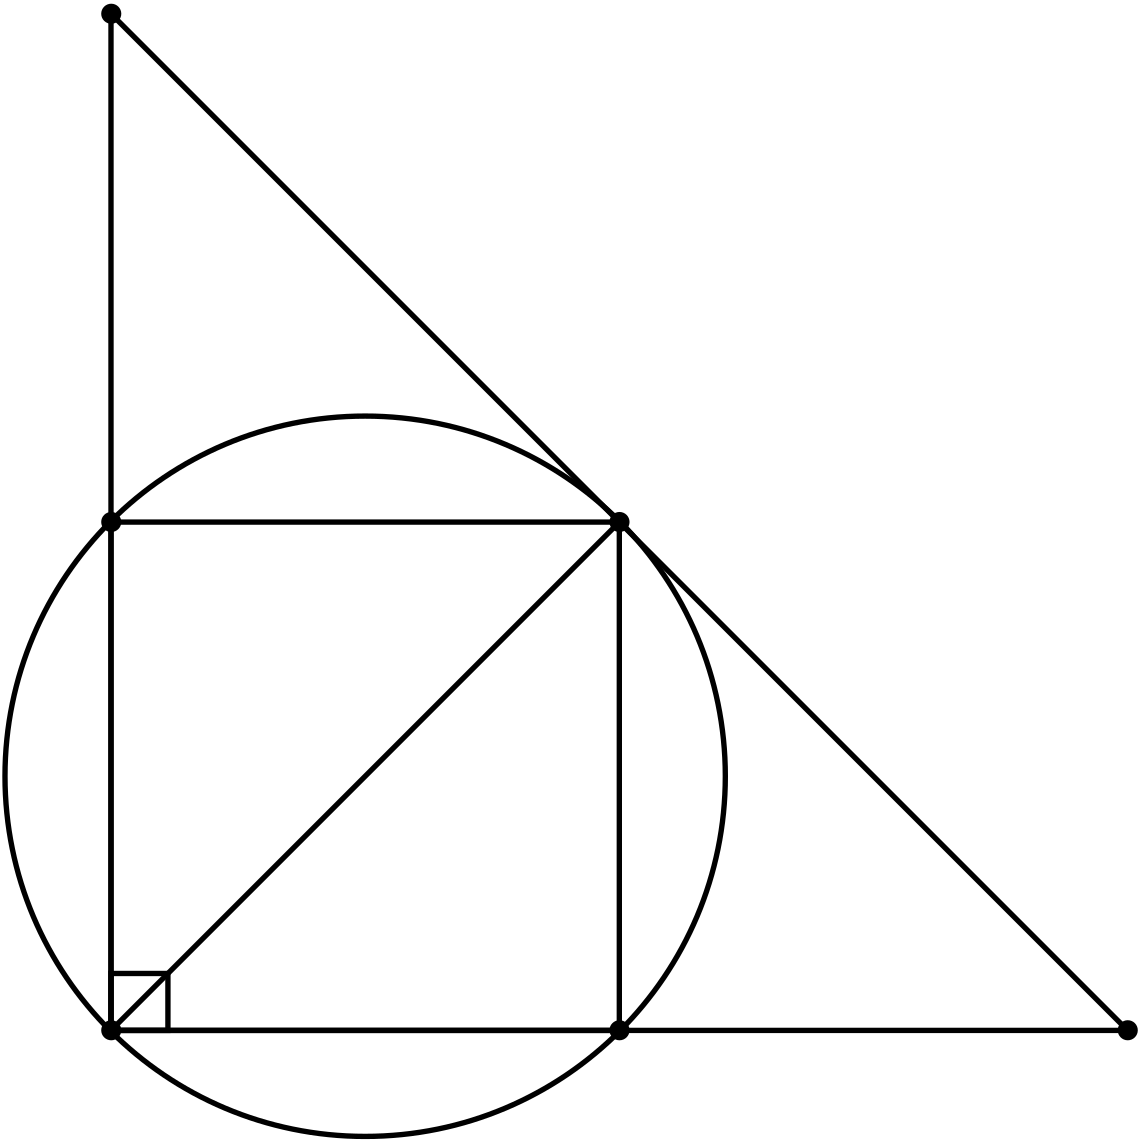
\includegraphics[height=12cm]{img/fig08.png}
\end{center}
\end{document}